
\documentclass[a4paper, 12pt]{article}

\usepackage[french]{babel} 
\usepackage[utf8]{inputenc}
\usepackage[T1]{fontenc} 
\usepackage{amsmath}
\usepackage[toc,page]{appendix}
\usepackage{amssymb}
\usepackage{listings}  
\usepackage{graphicx}
\usepackage[margin=2.5cm]{geometry}
\usepackage{amsmath,amsfonts,amssymb}
\usepackage{hyperref}
\lstset{
language=Java,
breaklines=true
}



\newcommand*{\plogo}{\fbox{$\mathcal{PL}$}} % Generic publisher logo

%----------------------------------------------------------------------------------------
%	TITLE PAGE
%----------------------------------------------------------------------------------------

\newcommand*{\titleGM}{\begingroup % Create the command for including the title page in the document
\hbox{ % Horizontal box
\hspace*{0.2\textwidth} % Whitespace to the left of the title page
\rule{2pt}{\textheight} % Vertical line
\hspace*{0.05\textwidth} % Whitespace between the vertical line and title page text
\parbox[b]{0.75\textwidth}{ % Paragraph box which restricts text to less than the width of the page

{\noindent\Huge\bfseries Software Project\\ Engineering }\\[2\baselineskip] % Title
{\Large \textit{Final Report}}\\[4\baselineskip] % Tagline or further description
{\Large \textbf{Project leader} : Hélène Verhaeghe}
\\
{\Large \textsc{\textbf{Group E}}\\\textsc{Aurian De Potter(Group leader)},\\ \textsc{Eddy Ndizera},\\ \textsc{Ivan Ahad},\\ \textsc{Arnaud Dethise},\\ \textsc{Ludovic Fastré},\\ \textsc{Anthony Dechamps},\\ \textsc{Geoffroy Husson},\\ \textsc{Jonathan Legat}} % Author name

\vspace{0.5\textheight} % Whitespace between the title block and the publisher
{\noindent \Large \textbf{INGI2255}}\\[\baselineskip] % Publisher and logo
}\\

}
\endgroup}


\clearpage
\setcounter{page}{0}
\begin{document}
\titleGM
\section{Introduction \& Presentation of The Project}
We will start the \textit{Phase 4} report by a summary of our meeting with the client. We will then explain how the implementation of the requirements planned for this phase is going, and give information about the evolution of the architecture of our program. For this phase, we had to submit our code to the project. It is available in section 3.3, by following our GitHub repository.
\newpage
\section{List of All The Requirements}
We will now list all the elements that we were asked to implement in our software. The requirements had different priorities, divided into \textit{Must Have, Should Have, Could Have and Nice to Have}. However, rather than dividing them in those four categories, we decided to divide them into mandatory requirements and optional ones (the optional ones are in italic). We also sorted  them depending on if they're functionnal or non-functional. Note that we added some requirements not explicitly said by the clients but that we consider to be relevant for the project (such the privacy parts).

\textbf{Functional} :

\begin{itemize}

	\item User : 
	
	\begin{itemize}
		\item The user can enter his data (including special characters) 
		\item The users can register to a tournament as a pair, selecting his category 
		\item \textit{The user can reuse old data linked to his email address to automatically fill a registration form}
		\item The user can register for activities during a tournament (barbecue, etc) and choose preferences such as taking responsibilities and payment method
		\item \textit{The user can register on a tournament alone and be matched with another player}
		\item The user can register a personal court as being available for the tournament
		\item \textit{Users who registered their own court can see information about players who will play on those.}
		\item \textit{The user can use a payment method among several options}
		\item The user can leave a comment when registering
	\end{itemize}

    \item Admin : 
    
    \begin{itemize}
    	\item An admin can start or close a tournament
    	\item An admin can close the registration for a tournament (and trigger the creation of pools)
    	\item An admin can create an admin account
		\item An admin can create a staff account
		\item An admin can delete an account

    \end{itemize}
    
    \item Staff : 
    
    \begin{itemize}
    	\item After a pool has been generated, a staff member can manually reorganize it
		\item A staff member can manually assign a court for each match, or modify it in case of raining
		\item A staff member can use a mail list / newsletter functionality
		\item A staff member can enter or edit match result data
		\item A staff member can see all the user informations (except credentials)
		\item A staff member can visualize and print the evolution of the tournament in a fashionable and displayable form (both graphic and text), step by step using the knockoff, and print the pool matchup sheet
		\item A staff member can access the courts list
		\item \textit{A staff member can manually match two users as a pair for a tournament}
		\item \textit{Common page for staff members}
		\item \textit{Files sharing between staff members}
		\item \textit{Communication channel between staff members}
    \end{itemize}
    
     \item System :   
     
    \begin{itemize}
    	\item \textit{The system can create pools and match ups}
		\item \textit{The system must confirm email addresses}
		\item \textit{The system must query AFT rankings}
		\item \textit{The system can create smaller pools when it rains}
    \end{itemize}
    
\end{itemize}

\textbf{Nonfunctional} :
\begin{itemize}


	\item Interface :
	
	\begin{itemize}
		\item The interface must be user friendly
		\item \textit{The interface must be mobile friendly}
	\end{itemize}

	\item Documentation :
	
	\begin{itemize}
		\item The software must be well documented

	\end{itemize}
	
    Privacy :
    
    \begin{itemize}
    	\item Turn off indexation of private data

    \end{itemize}



\item Reasons to use a new software :


	\begin{itemize}
		\item Interface is easier to use
		\item Many tasks are automated
		\item Code base is simpler and more modular if future modifications are wanted
		\item More flexibility for users such as solo enrollment
	\end{itemize}

\end{itemize}
\newpage
\section{Development of the project and Implementation}

The requirements below are the ones we planned to develop for the second phase. This time, every requirement has been implemented. \\
\subsection{For this phase}
	
\begin{itemize}
 
\item Files sharing between staff members (Eddy, Aurian)
\item Communication channel between staff members (Eddy)
\item The user can use a payment method among several options (Aurian)
\item The system must query AFT rankings (Optional)(See below)
\item The system can create smaller pools when it rains (Optional)(See below)
\\
\end{itemize}

It is important to note that the requirements haven't been implemented in this particular order.\\

You can see in the list above who implemented which requirement(s) for this phase. 

\subsection{Implementation \& choices}

Here are a few other features that we implemented during this phase. \\

Upon encoding all the scores of the matches in a pool, the winner of this group is displayed in green and the knock-off tournament is created in the database. Plus, it is now possible to see the bracket with a pretty graphical version. The players that are the winners of a group will then get to the bracket. The scores are, for now, only editable by an admin account. Another feature that was added is that a user can now delete his own email address from the database, so that he can delete his own information on his own.\\

For the implementation of \textit{"The system must query AFT rankings" and "The system can create smaller pools when it rains"}, as these two functionalities were optional, we decided not to implement them. It thought it would take too much time to do so, and that implementing wouldn't be a great benefit after all.\\

As you can see, there weren't many requirements as scheduled for this phase. As stated in the previous report, this phase was much more dedicated to improving some underlying functionalities of the website to make it easier to use.

\subsubsection*{Implementations according to meeting with client}

First of all, as requested, we implemented a system that allows to exchange messages. We also added a system that allows to share files that they can upload/download. The staff members already have other means to communicate, so these two features are important for very important announcements. They are available on a dedicated page. You can see in figure \ref{annonce} below how a staff member can put an announcement, and how one can upload files in figure \ref{file} \\
\begin{figure}[h]
  \caption{\label{annonce} Announcement creation}
  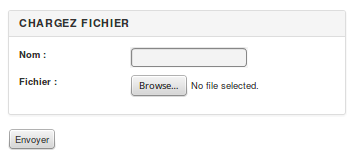
\includegraphics[scale=0.7]{annonce.png}
\end{figure}
\begin{figure}[h]
  \caption{\label{file} File sharing}
  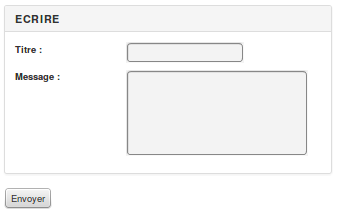
\includegraphics[scale=0.7]{fichier.png}
\end{figure}


It is also now possible to modify the pools by taking into account the commentaries made.\\

We also added a functionality that allows to look for players and courts, but also pairs. We then added a list of all the players and all the courts.

\subsubsection*{Changes during registration}
Secondly, we focused on modifying the registration of a player, as it was asked by the client. We have implemented the smart registration, where a player is automatically assigned to a tournament according to his information.\\

Moreover, when a form is filled, there is a summary of all the player information, allowing him to check what he is going to pay afterwards. You can see in figure \ref{recap} how the information is presented after validation.

\begin{figure}[h]
  \caption{\label{recap} Summary of player information}
  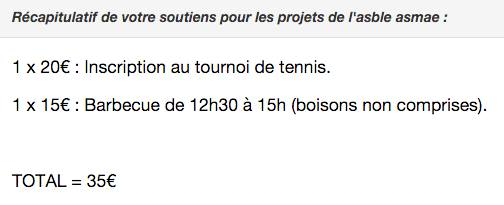
\includegraphics[scale=0.7]{recap.png}
\end{figure}

Another modification is that now the payment choice is chosen after a user has entered and validated all his information.
\subsubsection*{Bugs fixed}
In the last sprint, it was said in the previous report that the staff member interface had a different background to differenciate the navigation between a simple user and a staff user. We actually submitted a wrong live version where this feature was not implemented yet, which is now fixed.\\

One bigger issue was that we implemented a functionality that allowed to use an email so that a user doesn't have to fill all his information. By using the email, the system retrieved all the information from a past registration. However, this feature lead to information leak. From that point, we had to make a decision : we decided to send a confirmation email with a link, this link sends a token that allows the user to be recognized and to display his information. It is important to notice that in the case of a pair, only the information of the one who entered his email will be displayed, the other one will have to manually fill his form. It is a choice to have a more secured system, especially when two players are joined as a pair and if they're unknown to each other. We decided to implement this functionality in the last phase.\\

Some other bugs such as getting an error when trying to modify a user while being logged as a staff member, or one player couldn’t register alone leading to an error, or when logged as staff member when clicking on a tournament it changed to a user tournament. Those problems have all been fixed as well.

\subsection{The software}


Here is the live version of our website : http://sep2015e.herokuapp.com.  To get admin access you should add "/admin" in the url.\\

\textbf{To get access to the code of our project}, you can click on the link to our \textit{Github} repository : https://github.com/ivanahad/sep2015E\\
\subsubsection*{How to modify a tournament}

\section{For next phase}
\subsection{Tests to improve the software}
To improve our software, we are going to ask random people to test the website to see if it is user-friendly and easy to use, and then we will proceed to modify it accordingly.\\

We will also navigate randomly to search for bugs and strange behaviors that may arise after modifications of the database.\\
 
We will also test our website on different monitors with different screen sizes to see if it fits the window correctly.\\

\subsection{Documentation}
The documentation will be one of our main focuses. It will be divided into two parts: the first will be dedicated for the staff and admin and the second for the maintainer of the website. For the admin and staffs, the documentation will be a guide on how to navigate on the website and on how to basic stuffs like as modifying a pool, editing a player, etc. This documentation will be found on a wiki but links will be on the website to directly access the content specific to a part of the website. For the maintainer of the code, the documentation will be more technical. We will explain our implementaion, what we use and how we do it. 



\newpage
\section{Architecture discussion, choices \& UML Diagram}

You can see our UML diagram in Figure 4. Since the last phase, we changed.\\

In the architecture, in this phase, there isn't much that has changed. However, one big change is that we added many methods that now allow to modify information about users, courts, tournaments, etc. Making things changeable manually was one of our main coucerns for this phase, as it was requested by the client.

\begin{figure}[b]
	\centering
 	\caption{\label{uml} UML diagram}
	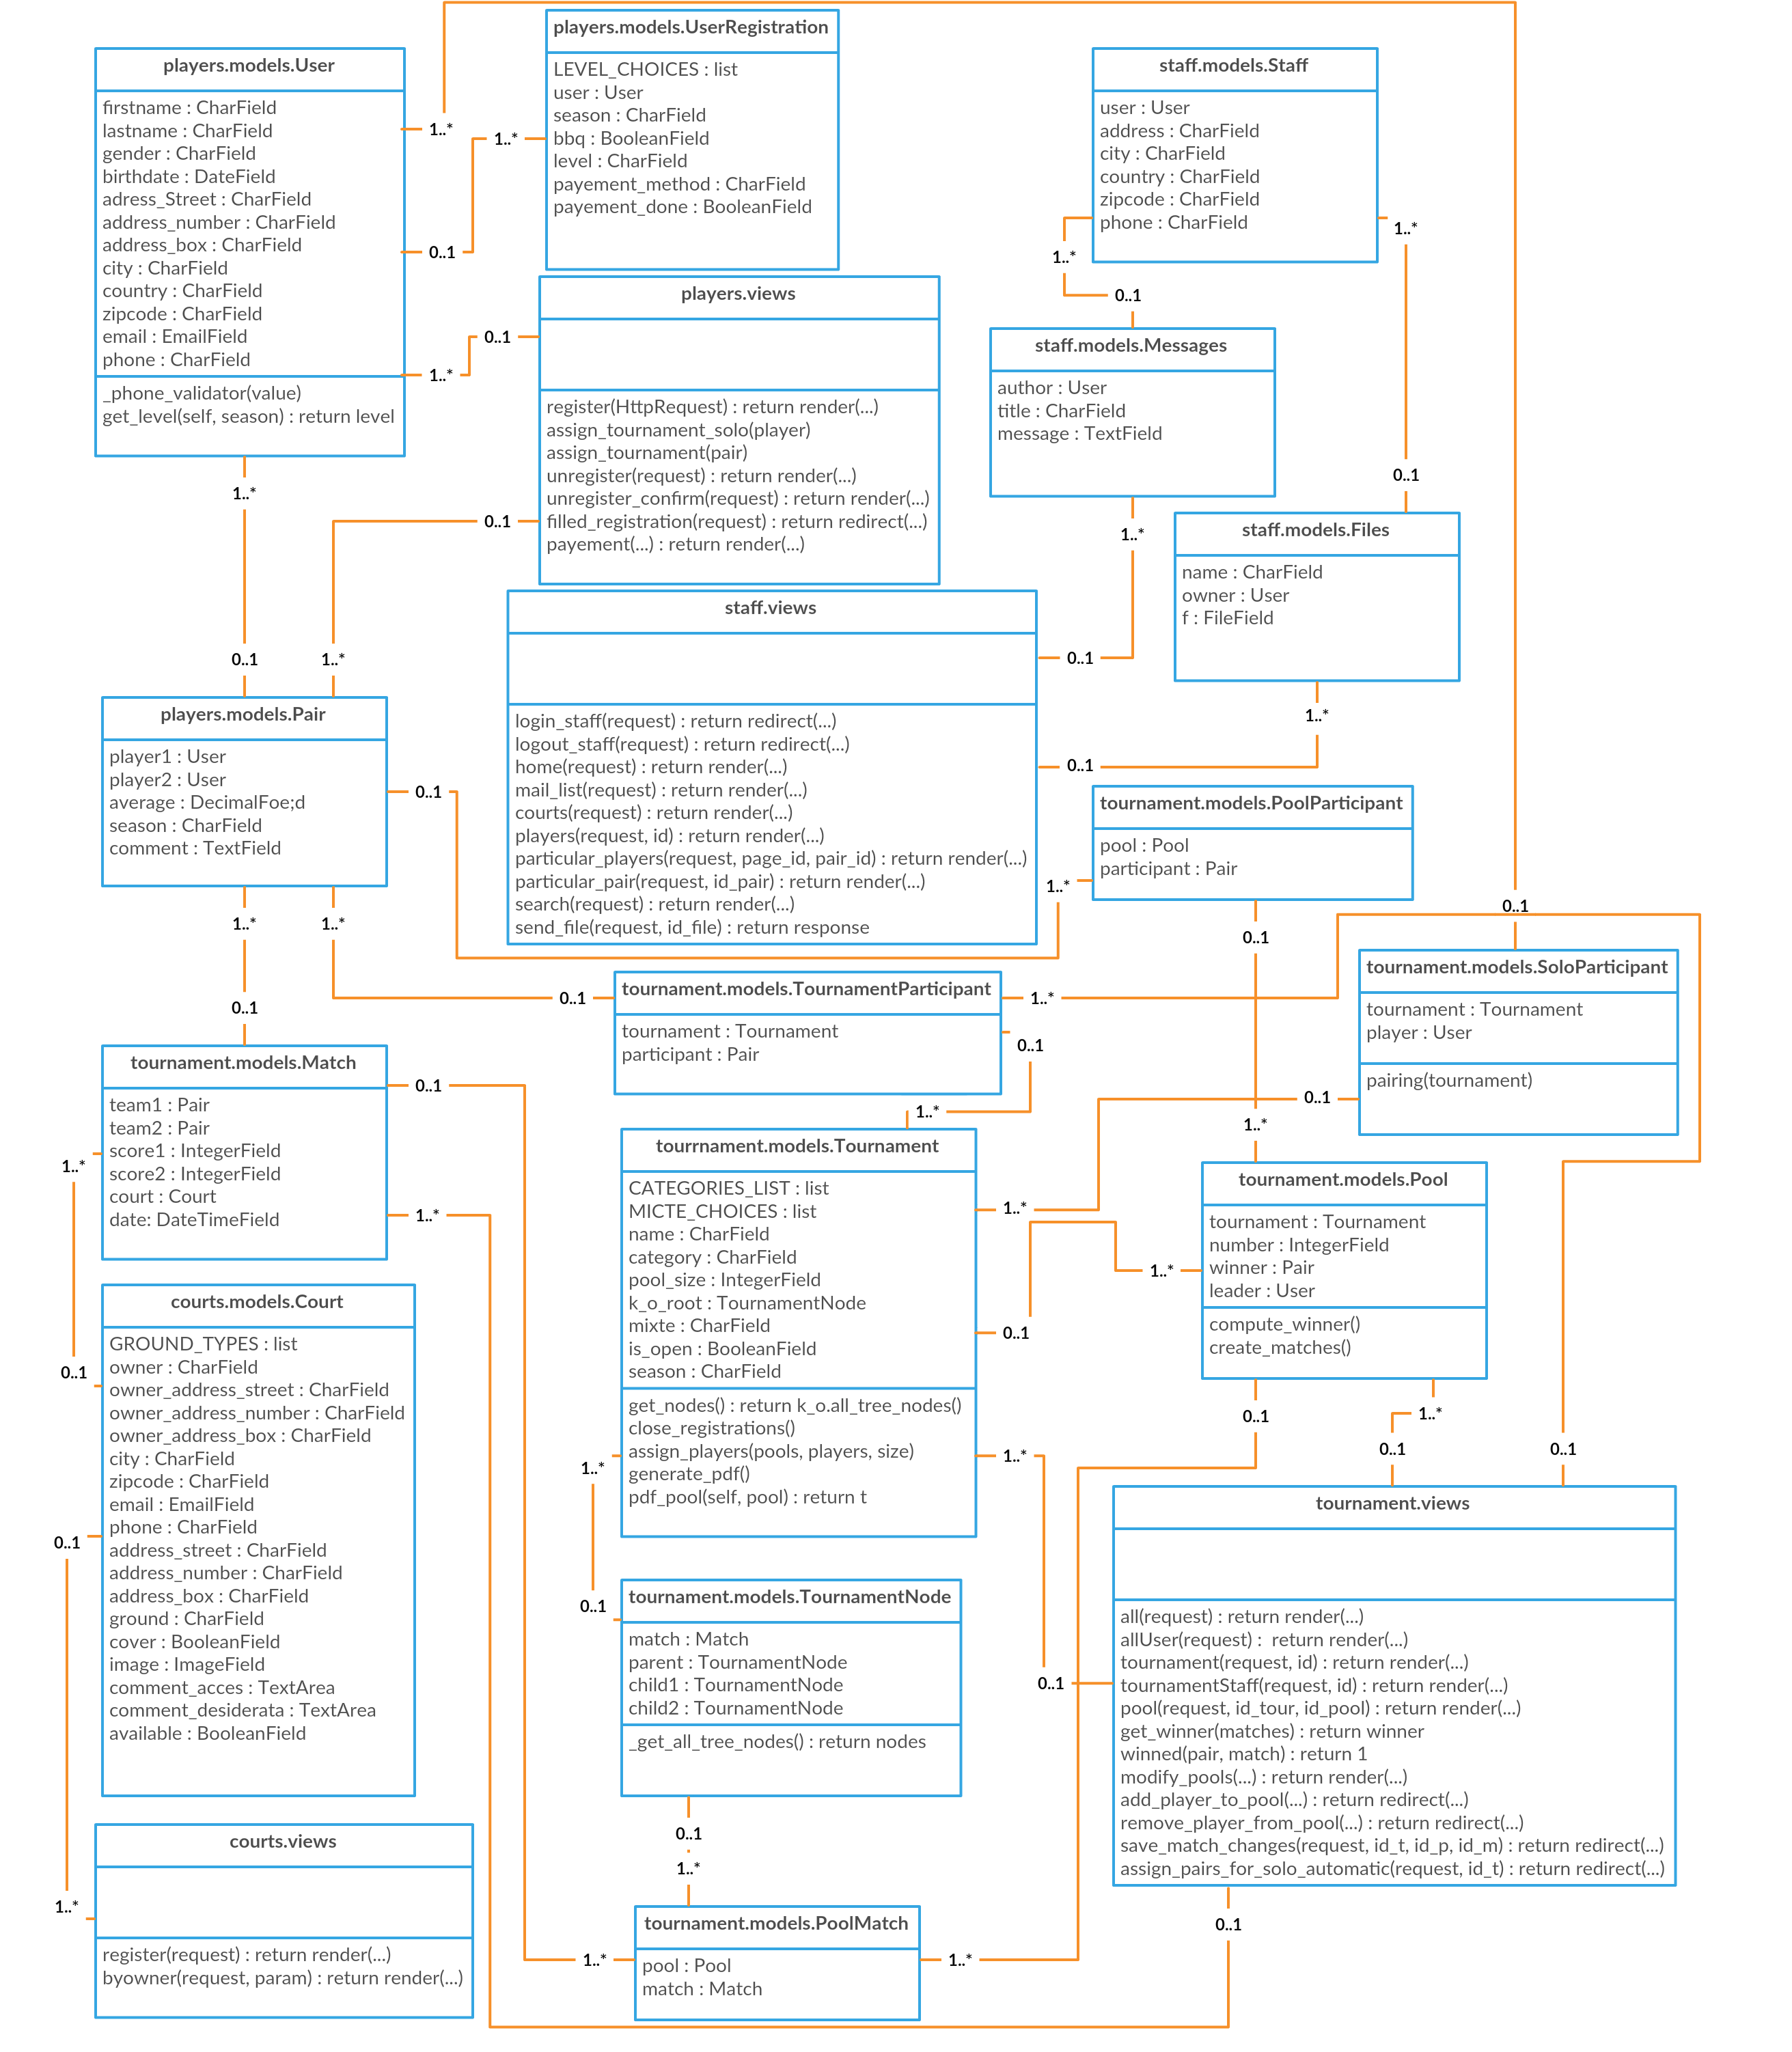
\includegraphics[scale=0.2]{Class.png}
\end{figure}

\subsection*{Sequences diagram}

You can see in figure \ref{playerseq} the sequence diagram for how a player registers to a tournament with an email confirmation. It has been updated since the last phase's report.

\begin{figure}[position]
   \caption{\label{playerseq} Sequence diagram}
  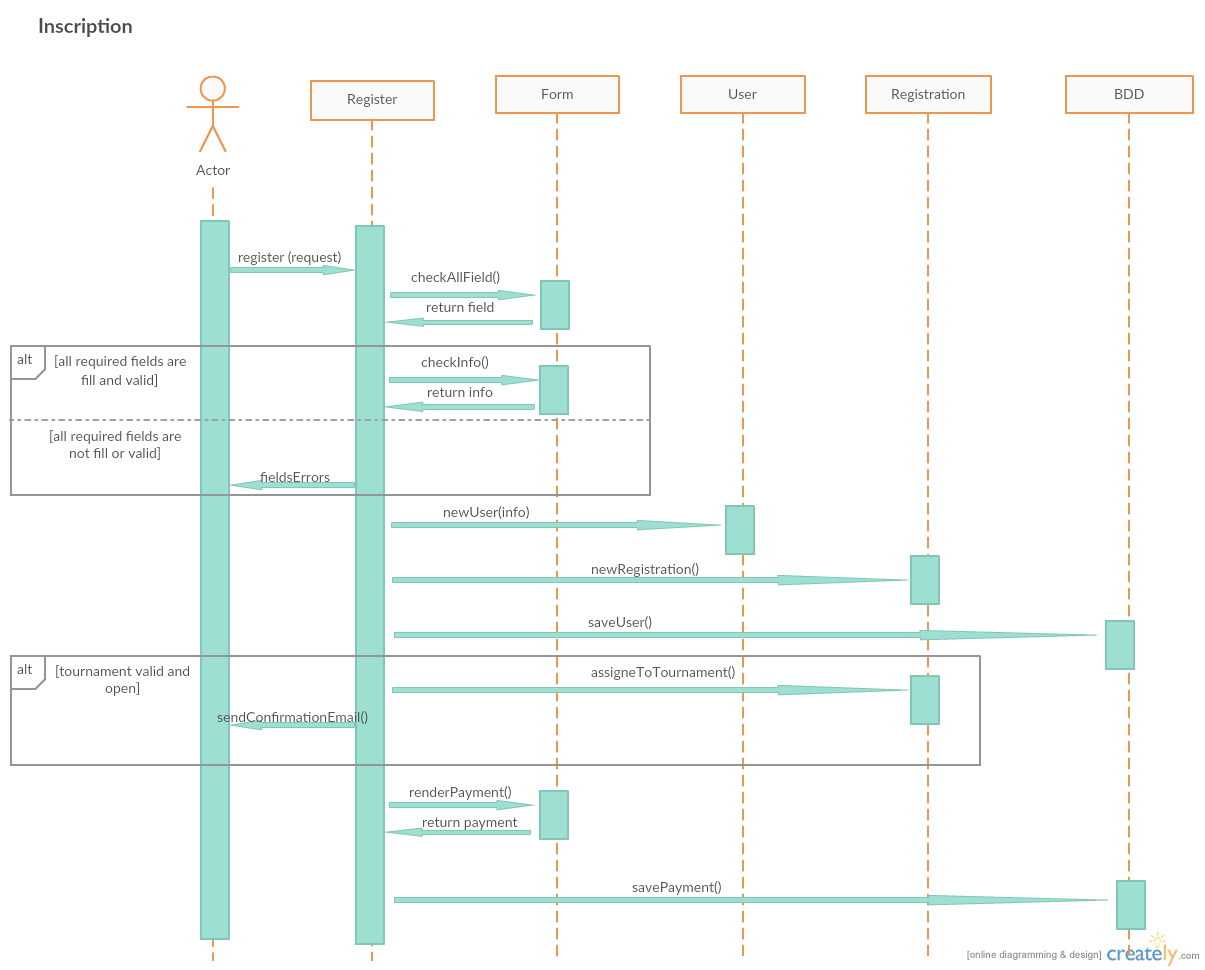
\includegraphics[scale=0.4]{Inscription.png}
\end{figure}

The second sequence diagram describes the life cycle of a tournament, how players are added into groups, how the knock-off tournament is created, how the tournament is created, etc. 

\begin{figure}[position]
   \caption{\label{tournseq} Sequence diagram for tournament}
  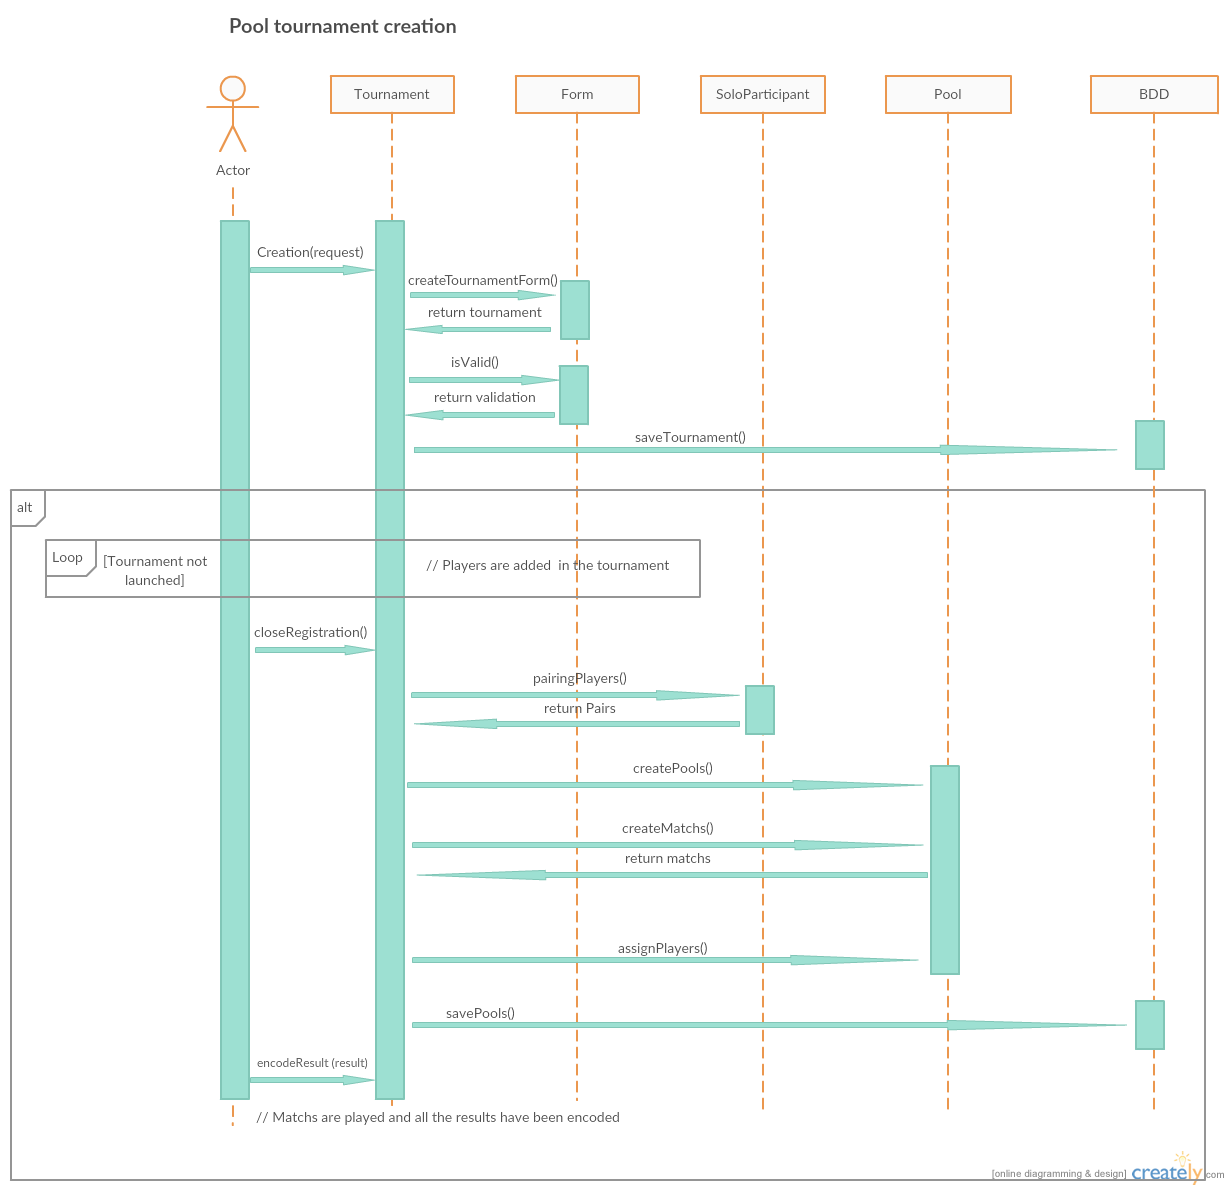
\includegraphics[scale=0.4]{Tournament.png}
\end{figure}


\section{Software development method}

We are briefly going to explain the way the group is going to develop the project. After being introduced to the project by our customers, we had to choose between a few development methods to use throughout the making of the project. The group then picked the \textbf{Agile} method. \\

The first step of this method is writing down user stories. These are used to present all the functionalities of the software which is the website. Afterwards, the group has to discuss about the importance and the difficulty of each user story, and then decide which of them have the top priority. \\

When this is done, we will use a kanban to organize the process of the project. The kanban contains all the user stories, and is divided into the following categories : “To do, doing this iteration, done this iteration, and done”. Every member of the group picks the user stories he thinks he is able to implement, so it allows us to know which member has done each task. For the kanban we will use the Trello Website. \\

The programming language used will be Python, with the \textbf{Django} framework. We will use the third version of Python, and the 1.8 version of Django. Lastly, we will use the \textbf{Bootstrap} framework for the design of the website ( the css part essentially). \\

To easily share the project’s code, we will use a Control Version System, which is in this case \textbf{Mercurial}. Mercurial, and its underlying service called BitBucket, is preferred since it allows us to make private repositories. 

We also decided to divide the project into 4 iterations, corresponding to the 4 phases presented to us. With the Agile method, there will be a working deliverable for each of these phases. Through each iteration, we will have to add up functionalities to the working project, until each of them is implemented.  \\

There are a few reasons why we picked this way of working. First of all, this method was genuinely our first choice since it is the one we are the most comfortable with, as we have been using such a method for a few projects now. Moreover, we liked its versatility since every member of the group has to be involved in every aspect of the project. Furthermore, after each iteration, we will have a meeting with our Assistant. This meeting will allow us to get a feedback of each deliverable. The feedback received will then help us to know if changes need to be done, if there are unnecessary things, or if our project is moving towards the right direction. Finally, with the Agile method, we will first implement all the “must have” functionalities, which allow us to focus on the core of the software, and then add up the functionalities with less priority. \\

\section{Planning}



\section{Requirement analysis}


\section{Use cases}

Here are a few use cases showing how our website will react upon receiving an action (registration of a player, registration of the owner of a court and creation of a group). Note that those use cases are subject to change when developping the project but it gives a good idea about the general process.\\

\textbf{Registration of a player}

\begin{itemize}
	\item The admin enables the registration for a tournament.
	\item The user must access the registration page.
	\item The user fill his personal informations on the page.
	\item Or load the from previously used email address. 
	\item The user must enter the personal information of his tennis partner if he plays in duo.
	\item The user gets a confirmation email. (Past this point he must contact the staff/admin to modify his information.)
	\item The admin closes the registration just before the tournament.
\end{itemize}



\textbf{Registration of the owner of a court}

\begin{itemize}
	\item The owner must access the registration page.
	\item The own fill his court informations on the page.
	\item The owner receive an email confirmation.
	\item When the admin opens a new tournament, he will be notified of all the previously used courts and asks the owners about their availability.
	\item The staff will check the court and mark it as suitable.
	\item When a court is assigned to a tournament, the owner is notified by email.
\end{itemize}


\textbf{Creation of a group}

\begin{itemize}
	\item Once the registrations are closed, the system will generate the groups for each category.
	\item The staff will review the generated list. If there are wishes to fulfill, the list can be manually reorganized. At this step, the staff can also contact the users with payment issues.
	\item Once the groups are checked, the staff confirms their composition.
	\item The system sends an email to the users to inform them of the location and time of their matches and of their payment status. The leader is also informed of what is needed of him.
\end{itemize}

\section{Conclusion}

For this phase, we modified our software according to our meeting. We mainly focused on correcting bugs and making the website more user-friendly.

\end{document}